% To add an image or include a .tex file you need to add
% \CWD
% to the relative (to the main document) path.
%
% Example:

\begin{center}
\textit{Após inventar o avião, o grande mineiro Alberto Santos-Dumont precisava testar sua invenção.}
\end{center}

\begin{figure}[H]
  \centering
  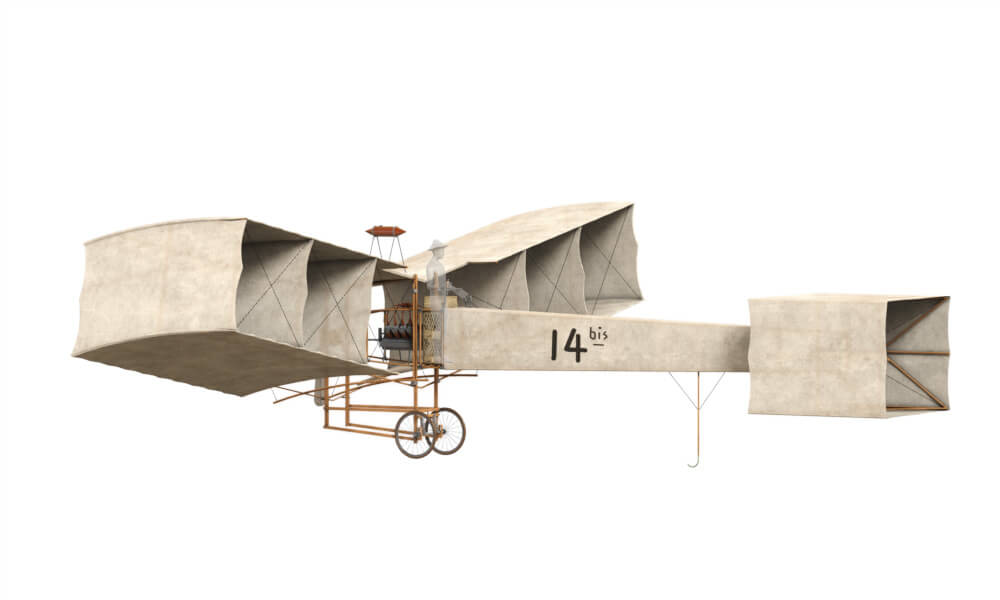
\includegraphics[width=7cm]{\CWD/14bis.jpg}
  \caption{14-bis, o primeiro avião da história a levantar voo.}
\end{figure}

Para melhorar as chances de decolar sua lendária aeronave, o 14-bis, Santos-Dumont precisava de uma pista de decolagem que fosse bastante reta e o mais comprida possível. Uma pista de decolagem é descrita como uma sequência de números (representando a altura de cada trecho da pista), que é considerada reta se a diferença em valor absoluto entre duas posições adjacentes nessa sequência não é maior que um (não queremos estragar o trem de pouso da nossa querida aeronave de papel com terrenos acidentados!).

Dado um mapa topográfico da área, descrito como uma matriz $N\times M$ (em que cada valor da matriz guarda a altura da posição), imprima o tamanho da maior pista de decolagem possível, sendo que as pistas de decolagem podem ser no sentido norte-sul (intervalo de uma coluna da matriz) ou leste-oeste (intervalo de uma linha da matriz).

\begin{figure}[H]
  \centering
  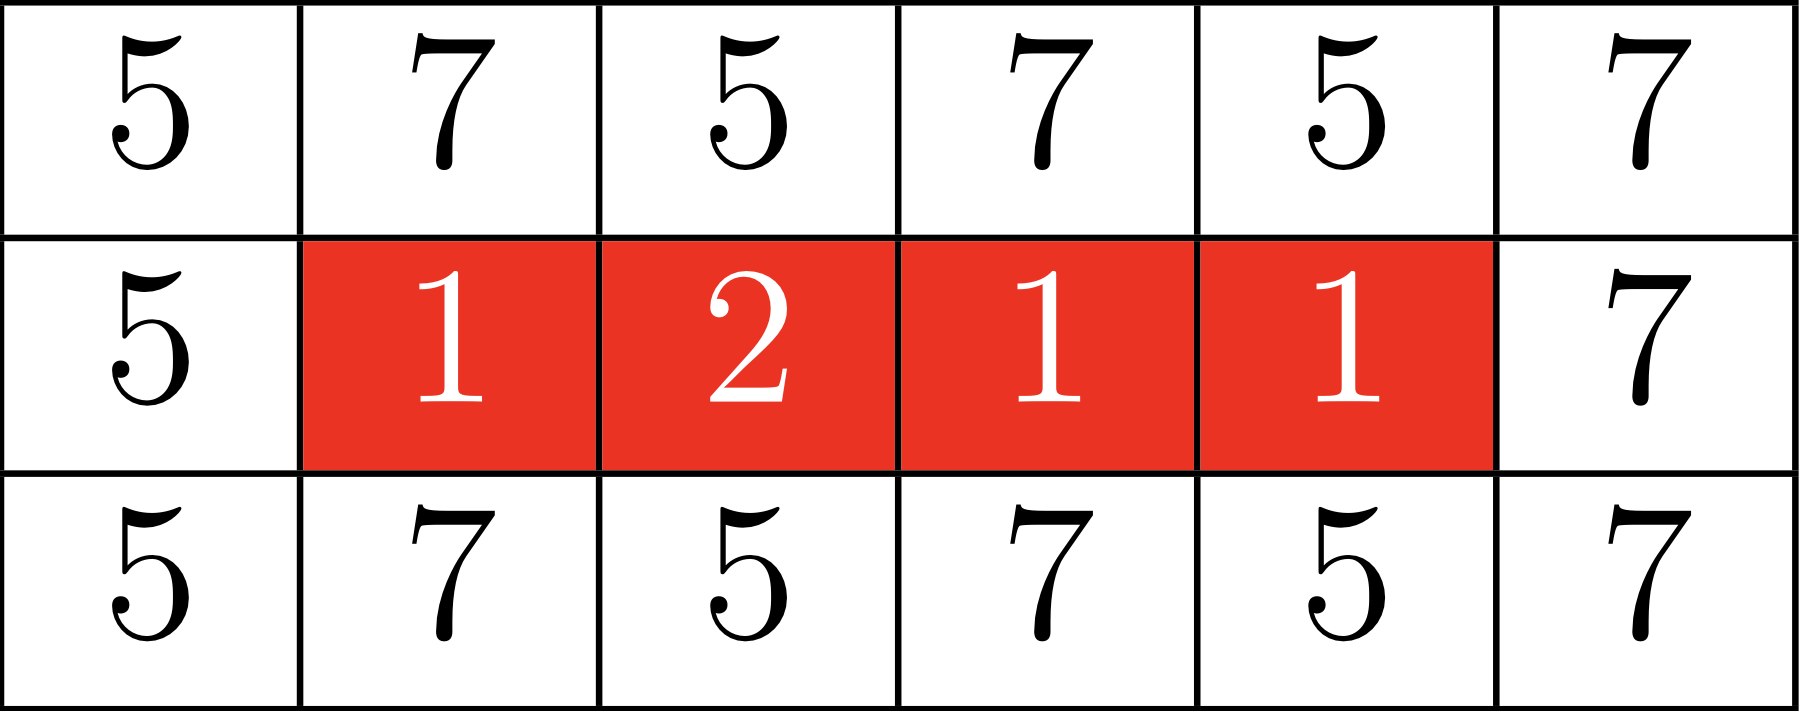
\includegraphics[width=7cm]{\CWD/matrix-sample.png}
  \caption{No exemplo $1$ a maior pista de decolagem está no sentido leste-oeste e tem comprimento $4$.}
\end{figure}
%
% For input, use one of the following
%
\section*{Entrada}

A primeira linha conterá dois números $N$ e $M$ (tais que $N \times M \leq 2\times 10^5$) que representam o número de linhas e colunas da matriz, respectivamente.

Depois disso teremos $N$ linhas. Na i-ésima delas teremos $M$ números $a_{i, 1}, \ldots, a_{i, M}$ onde $a_{i, j}$ representa o altura do terreno na linha $i$ e coluna $j$ da matriz e $0 \leq a_{i, j} \leq 10^9$.

%
% For output, use one of the following
%

\section*{Saída}

Imprima um número que representa o tamanho da maior pista de pouso para o 14-bis.

\section*{Restrições}

\begin{itemize}
  \item $N \times M \leq 2\times 10^5$.
  \item $0 \leq a_{i, j} \leq 10^9$.
\end{itemize}

%\sampleio will look for files named sample-n.in and sample-n.sol (where n is 1, 2, 3...)
%in the documents directory and include them as samples.

\exemplo
